% ----------------------------------------------------------
% Consciousness subsection
% ----------------------------------------------------------
\subsection{Consciousness}
A logical moment can be formed by a division (first moment) or by logical subdivisions (other moments).
	\begin{figure}[H]
	\caption{Logical interval}
	\label{fig:consciousness_logical_moments}
	\centering
	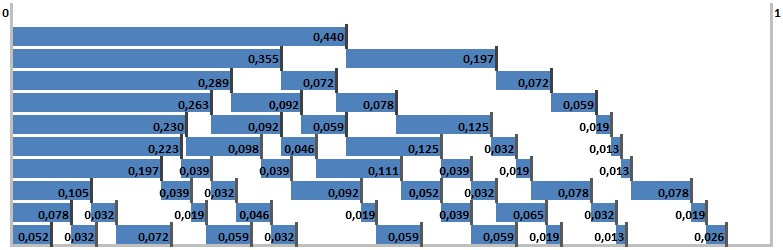
\includegraphics[scale=.7]{sections/images/consciousness_logical_moments.jpg}
	\floatfoot{Example of a logical interval with ten logical moments.}%\footnotemark}
	\end{figure}
	%\footnotetext{Fonte: note}

Consciousness is the logical moments of an expansion represented in its units.
	\begin{figure}[H]
	\caption{Conscious logical interval}
	\label{fig:consciousness}
	\centering
	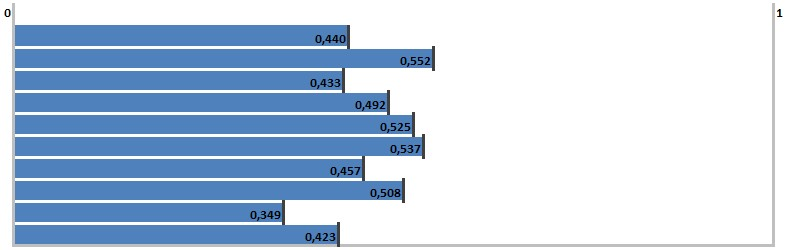
\includegraphics[scale=.7]{sections/images/consciousness.jpg}
	\floatfoot{Example of a conscious logical interval with ten units of logical moments.}%\footnotemark}
	\end{figure}
	%\footnotetext{Fonte: note}

It can be seen in Table \ref{tab:10000_all} that the probability of 99.99\% of the samples in a population (Range), which increase in quantity as the logical moments increase, tends to be increasingly in the center of the logical interval and this centralization tends to infinity.
	\begin{figure}[H]
	\caption{Centralization of 99.99\% of the samples}
	\label{fig:centering_of_99_range}
	\centering
	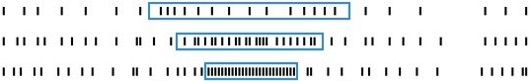
\includegraphics[scale=1]{sections/images/centering_of_99_range.jpg}
	\floatfoot{Tendency to center the range of 99.99\% of the samples.}%\footnotemark}
	\end{figure}
	%\footnotetext{Fonte: note}

Consciousness tends toward the representation of a logical wave, the largest logical wave in a population (a histogram of the normal distribution) as shown in the figure \ref{fig:trend_chart_of_normal_distribution}. All of the aspects listed below are inherent in the logical abstraction called consciousness.

\subsubsection{Infinite}
One of the most important aspects that the negation of nothingness brings (negation of self), is infinity, that is, in any logical interval the infinite fits again. The primordial logic that started the entire logical interval is the same found in its subsequent intervals (subintervals). This substantiates how a high-level logic like the human subconscious explains primordial logic, since it is not necessary to go back to the first logical moment of the interval to deduce it, as this phenomenon is omnipresent throughout the interval.

\subsubsection{Waves}
Probabilistically, the distribution of new samples from a population tends to concentrate more samples toward the median of the population as the frequency of samples increases in this direction. However, the distribution of these samples with uniform growth frequencies is infinitesimal compared to the random possibilities of this growth. Thus, the tendency of these growth frequencies toward the median, together with the very low (infinitesimal) probability of this growth being uniform, leads to frequencies in the waveform. The relationship of the density or amplitude of a wave to its length is detailed in the next subsection.
	\begin{figure}[H]
	\caption{Waveform}
	\label{fig:consciousness_waves}
	\centering
	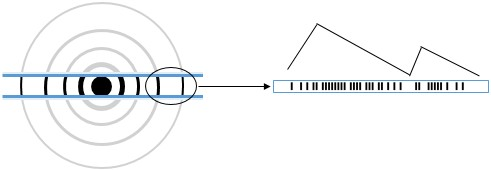
\includegraphics[scale=.8]{sections/images/consciousness_waves.jpg}
	\floatfoot{Wave pattern inferred by the trend of this distribution with higher frequencies towards the population median and very low probability of uniform growth of these frequencies.}%\footnotemark}
	\end{figure}
	%\footnotetext{Fonte: note}

Merging one wave into another eliminates its discrepancy and makes that wave cease to exist and become part of the first wave, which has its peak closer to the median, in this example. A wave doesn't die, it just merges with another wave closer to it.
	\begin{figure}[H]
	\caption{Wave unification}
	\label{fig:consciousness_uniform_wave}
	\centering
	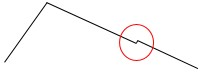
\includegraphics[scale=1]{sections/images/consciousness_uniform_wave.jpg}
	\floatfoot{Waves being unified to exemplify the uniform growth of the samples.}%\footnotemark}
	\end{figure}
	%\footnotetext{Fonte: note}

\subsubsubsection{Wavelength and Amplitude}
The histogram is used in the figures in this subsection and later to facilitate visualization and understanding of the distribution of samples in a population, because it represents very well the density curves of a population, according to the different views of the Figure \ref{fig:consciousness_wave_histogram}, representing only one interval or wavelength paired by the median of the population.  
	\begin{figure}[H]
	\caption{Histogram in different views}
	\label{fig:consciousness_wave_histogram}
	\centering
	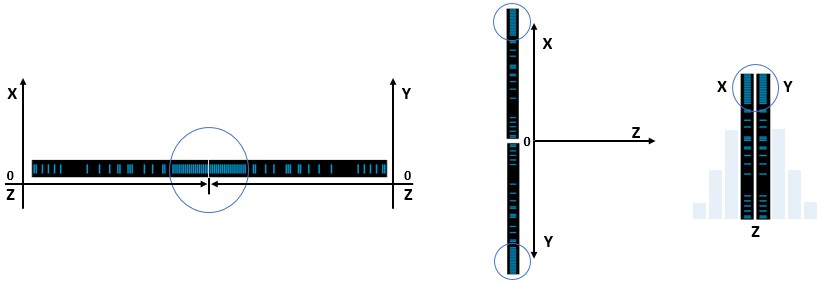
\includegraphics[scale=.7]{sections/images/consciousness_wave_histogram.jpg}
	\floatfoot{Different ways of population representation in a histogram.}%\footnotemark}
	\end{figure}
	%\footnotetext{Fonte: note}}
The length and amplitude of waves establish a quantity-per-interval or unit relationship. These units are established by wave entanglement, as seen in the next subsection. Thus, amplitude is the density of a wavelength, the density of some interval.  

When adding a new sample to the population, the entire interval is proportionally distributed to match that sample. When looking at the population at smaller intervals or wavelengths, their wave amplitudes will conform to the distribution of samples from these subintervals proportionally, as shown in Figure \ref{fig:consciousness_space_volume_amplitude}.
	\begin{figure}[H]
	\caption{Wavelength vs. Amplitude}
	\label{fig:consciousness_space_volume_amplitude}
	\centering
	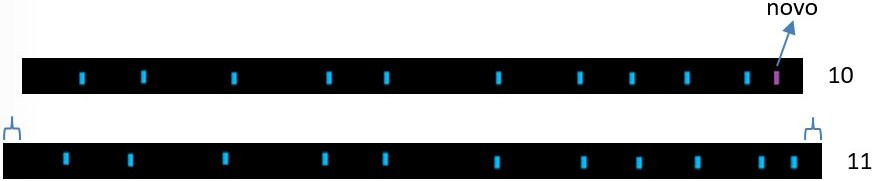
\includegraphics[scale=.4]{sections/images/consciousness_space_volume_amplitude.jpg}
	\floatfoot{Relationship of wave length and amplitude.}%\footnotemark}
	\end{figure}
	%\footnotetext{Fonte: note}}
	
Another important factor is the higher concentration of samples tend to be distributed at the peak of the interval, because the top of the subintervals or wavelengths that form the peak (histogram columns that form the highest point of the wave) are closer to the population median than the bottom of those wavelengths, as shown in the example in Figure \ref{fig:consciousness_space_amplitude_growth} in its center column in blue.
	\begin{figure}[H]
	\caption{Wave amplitude - peak}
	\label{fig:consciousness_space_amplitude_growth}
	\centering
	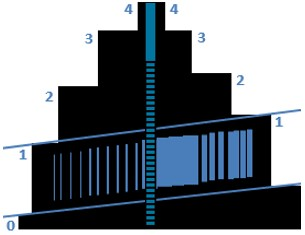
\includegraphics[scale=.6]{sections/images/consciousness_space_amplitude_growth.jpg}
	\floatfoot{Trend of the highest concentration of samples in the subintervals of a wave.}%\footnotemark}
	\end{figure}
	%\footnotetext{Fonte: note}}

In large intervals with many logical moments a smaller discrepancy of wave amplitudes is observed. In such intervals large systems of objects can be observed. The larger the intervals, the more balanced they grow towards the population median (probabilistically) as seen in Figure \ref{fig:consciousness_space_subconsciousness}. The lowest wave (dark blue) is the base wave of the system, that is, the wave that formed the other waves. Wave systems can be complex, having several nested waves, best visible in Figure \ref{fig:consciousness_gravitational_force_system}. More complex intervals with this feature can represent, for example, the universe, then galaxies, stars, planets, etc.
	\begin{figure}[H]
	\caption{Wave amplitude at large intervals or lengths}
	\label{fig:consciousness_space_subconsciousness}
	\centering
	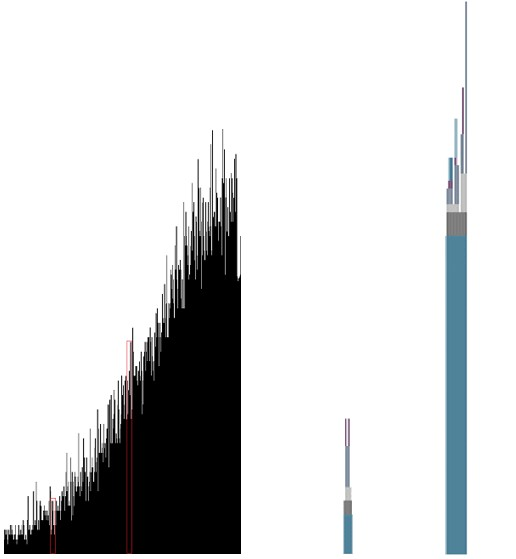
\includegraphics[scale=.45]{sections/images/consciousness_space_subconsciousness.jpg}
	\floatfoot{Smaller wave discrepancy at large intervals.}%\footnotemark}
	\end{figure}
	%\footnotetext{Fonte: note}

In smaller intervals and with many logical moments a greater discrepancy in wave amplitudes is observed. In these intervals smaller object systems can be observed. The smaller the intervals are, the more unbalanced they will grow towards the population median (probabilistically) as seen in the figure \ref{fig:consciousness_space_subconsciousness_min}. The lowest wave (dark blue) is the base wave of the system, that is, the wave that forms other waves. More complex wave systems with this feature can represent, for example, the atom, which is very small, present in huge quantities, and the particles orbiting its nucleus (electrons) are much more distant from it.
	\begin{figure}[H]
	\caption{Wave amplitude at small intervals or lengths}
	\label{fig:consciousness_space_subconsciousness_min}
	\centering
	
\includegraphics[scale=.45]{sections/images/consciousness_space_subconsciousness_min.jpg}
	\floatfoot{High wave discrepancy at small intervals.}%\footnotemark}
	\end{figure}
	%\footnotetext{Fonte: note}}

\subsubsubsection{Entanglement}
The most similar samples in terms of frequency and distribution are the samples that are part of the same wave. They are non-overlapping, opposite frequencies that complete each other.

Probabilistically, the two complementary parts of a wave tend to be at approximately equal distances, equidistant from the median, but this is not a rule and the complementary parts of a wave may be at different distances from the median. The phenomenon of parity of the parts of a wave is called wave entanglement.

These pairs tend to be formed by probability, where equal wavelengths have the same probability of samples distribution at two or more different points in the population. 

Intervals with similar temporal frequencies and spatial distributions are intervals formed by the same probabilistic unit, that is, intervals that have the same probabilistic scenario or context at a given logical moment. Being in the same probabilistic scenario (probabilistic units), these intervals have their samples in the same space-time scenario, which is called space-time lattice and is formed by the largest probabilistic unit in the population (all the samples in the population intermediated by the median). 

These entanglements form smaller waves (subconsciousnesses), similar to the largest wave in the entire interval, usually entangled by the population median (consciousness). Consciousness is the logic of the entire interval, while it forms subconsciousnesses or sub-logics, like small waves of a larger wave.These small waves are similar to the pattern of the larger wave.  Thus, a change in the larger wave (consciousness) are also changes in the smaller waves (subconsciousnesses) - a change that is induced indirectly by subconsciousnesses, analogous to the compression of gas in a cylinder, where by adding a new molecule of gas in the partially filled cylinder, closer or tighter these molecules will be inside it.  The opposite is also true, a new sample in a subconsciousness that is directly observed by it is also a change of the consciousness and will be induced indirectly by other subconsciousnesses, as shown in the figure \ref{fig:consciousness_space_volume_amplitude}.
	\begin{figure}[H]
	\caption{Subconsciousness}
	\label{fig:consciousness_subconscious}
	\centering
	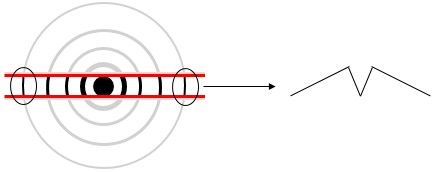
\includegraphics[scale=.8]{sections/images/consciousness_subconscious.jpg}
	\floatfoot{The wave pattern forms subconsciousnesses similar to the pattern created by consciousness, as seen in Figure \ref{fig:trend_chart_of_normal_distribution}.}%\footnotemark}
	\end{figure}
	%\footnotetext{Fonte: note}
	
The entanglement of waves can occur at different levels or intervals, as seen in Figure \ref{fig:consciousness_subconscious_entanglement}, which forms nested wave systems. Bordered braces identify intervals where a new sample triggered the jump (as seen in the next subsection), and bordered rectangles represent intervals that have been reordered. Borderless rectangles and braces represent the wave pair in the new order. The numbered arcs indicate the order of the jumps.

The largest entanglement is shown in the examples in Figure \ref{fig:consciousness_subconscious_entanglement} as the first jump or entanglement, which occurred when that interval was the smallest, probably.  Large intervals tend to be kept ordered by the reordering of their subintervals subsequently.The largest wave is commonly entangled by the population median.

The smaller intervals tend to get the entanglement first, and these reorderings caused by them allow the entanglement of pairs with larger intervals. Entangled pairs are the two opposite sides of a wave (peak or valley) and are entangled by its median, which may coincide with the population median when it is the largest probabilistic wave of the entire interval.
	\begin{figure}[H]
	\caption{Wave entanglement levels - wavelengths}
	\label{fig:consciousness_subconscious_entanglement}
	\centering
	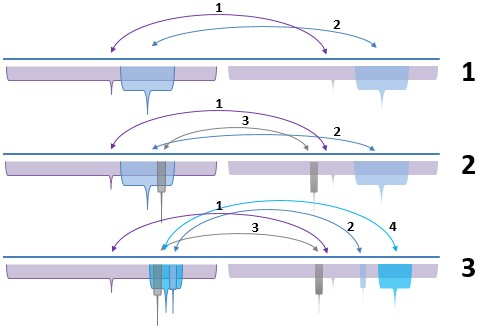
\includegraphics[scale=.8]{sections/images/consciousness_subconscious_entanglement.jpg}
	\floatfoot{Examples of entanglement levels of waves or levels of wavelengths.}%\footnotemark}
	\end{figure}
	%\footnotetext{Fonte: note}

The examples in Figure \ref{fig:consciousness_subconscious_entanglement} show the subintervals (peaks or valleys) entangled most strongly with other non-equidistant subintervals. Entanglements are closely linked to the wavelengths of a population. The possible wavelengths of a population are defined by these levels of wave entanglement. Thus, regardless of the order of the jumps, larger entanglements are the longer wavelengths and smaller entanglements are the shorter wavelengths, which allows larger waves to have smaller subwaves. 

The jump is a reordering done by the entanglement of waves to maintain the equivalent pairs, this reordering occurs only at the entanglement levels, not changing the order of the population samples. Thus, an entangled interval tends to return to a higher entanglement level as the probability of samples from that interval transitions temporarily between the valley and the peak towards equilibrium.

\subsubsubsection{Jump}
The jump is a reordering done by wave entanglement, as the samples of the entangled pairs are no longer equivalent with the addition of new samples from one side of the pair. The jump occurs on one side of a pair of waves and is a reordering, that is, both the part of the interval that has just received the new sample must better match the intended interval for the jump, as well as the reverse.

In Figure \ref{fig:consciousness_space_subconscious_observation_jump} the entanglement of waves (represented by columns of a histogram to facilitate the visualization of the interval) is observed. The reordering made by the entanglement causes a jump in the coordinates (X, Y and Z) according to the Space subsection.
	\begin{figure}[H]
	\caption{Reordering - jump}
	\label{fig:consciousness_space_subconscious_observation_jump}
	\centering
	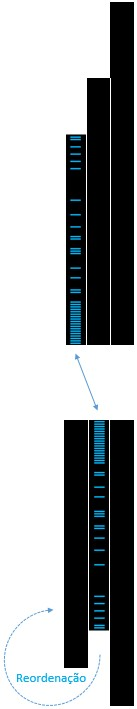
\includegraphics[scale=.53]{sections/images/consciousness_space_subconscious_observation_jump.jpg}
	\floatfoot{Jump caused by non-equivalence of the entangled pair with the addition of new samples on one of its sides.}%\footnotemark}
	\end{figure}
	%\footnotetext{Fonte: note}

Reordering of the jump occurs only at the entanglement levels, not changing the order of the population samples. An entangled interval tends to transition between entanglement levels as the probability of samples from that interval transitioning temporarily between the valley and the peak to equilibrium. Thus, the probabilistic tendency is that, for example, the electron that jumped from its origin orbit returns to this one as more samples are added to that atom's population interval, restoring its probabilistic character.

A photon, for example, enters the atom and electron as they move toward their reference lines, as shown by the blue sample to the right of wave 1 in Figure \ref{fig:consciousness_jump_photon.jpg}. The output of the photon from the electron and atom occurs similarly to the input, as new samples are added to the lower level wave the level of the lower level wave rises (the probability tries to normalize the peaks of the samples) and the samples that were once of the upper wave become of the lower wave.
	\begin{figure}[H]
	\caption{Atomic energy exchange}
	\label{fig:consciousness_jump_photon.jpg}
	\centering
	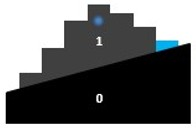
\includegraphics[scale=.8]{sections/images/consciousness_jump_photon.jpg}
	\floatfoot{How energy or new samples enter and exit an atom and electron.}%\footnotemark}
	\end{figure}
	%\footnotetext{Fonte: note}
	
\subsubsection{Time}
Time is the addition of new logical moments between existing moments as the self-negation of primordial logic proceeds. The changes are cumulative and as the number of logical moments increases, the less relevant each new moment within the conscious interval will be. One in a hundred is more relevant than one in a thousand. 
	\begin{figure}[H]
	\caption{Time}
	\label{fig:consciousness_time}
	\centering
	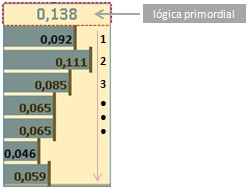
\includegraphics[scale=.8]{sections/images/consciousness_time.jpg}
	\floatfoot{Progression of time as logical moments advance.}%\footnotemark}
	\end{figure}
	%\footnotetext{Fonte: note}

In the introduction to this paper it was presented that primordial logic is a sequence of negations of itself at time zero, that is, at no time between its negations does logic [being], guaranteeing the primordial premise of the logical constant, [NOT BEING]. Thus, logic is an infinite, simultaneous and generalized sequence, a constant. In the observer-driven experience of time, the ordering of each sequence is the essence of this logical quantity and therefore more relevant than its origin, which is of a simultaneous nature, transcending time.

Each population has a different order in its sequence and it is this order that gives rise to the logical quantity called time. It is this order of the universe or of consciousness that will give the notion of what happens before or after, that is, the past, the present and the probabilistic future prospections.

Another important factor when observing time (the observer is more detailed in the consciousness subsection – Observer and life) is that, probabilistically, subconsciousnesses or intervals closer to the population median will have a larger addition of new samples in their intervals, which are directly observed by these subconsciousnesses. On the other hand, subconsciousnesses far from the population median will have a smaller addition of samples in their intervals and are subject to a larger number of indirectly induced changes, as shown in Figure \ref{fig:consciousness_subconscious}.  This phenomenon of temporal observation provided by the probability of the population distribution avoids the twin paradox \cite{twin_paradox}.

Prospections of the observer's future are based on the probabilistic distribution of the population and, therefore, on the probabilistic distribution of each sub-interval of the population. The universe tends to be probabilistic, while random at levels of detail (which makes events different), yet predictable at some level, as shown in Figures \ref{fig:consciousness_logical_moments} and \ref{fig:consciousness}. 

\subsubsection{Space}
In Figure \ref{fig:consciousness_space_waves}, the sample density of a population is shown, where pairs tending to the same probabilistic distribution are placed side by side and represented in histogram form. The formation of these pairs comes from wave entanglement.
	\begin{figure}[H]
	\caption{Entangled pairs represented in three spatial dimensions}
	\label{fig:consciousness_space_waves}
	\centering
	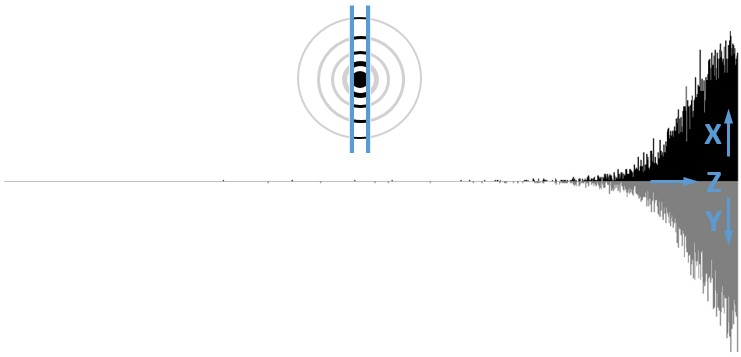
\includegraphics[scale=.7]{sections/images/consciousness_space_waves.jpg}
	\floatfoot{Example of entangled waves, represented in histogram form and obtained by the Logic\_WavePattern algorithm. \footnotemark}
	\end{figure}
	\footnotetext{The Logic\_WavePattern algorithm can be seen in Appendix \ref{app:algorithms}.}

The area grows quadratically to the increase in the amplitude of a wave (columns of the histogram), since the jump caused by the entanglement of the waves and the probabilistic distribution of samples in the interval naturally tend to maintain an equivalent growth in the pairs that form a wave. This aspect configures the inverse square law, which will be further explored in the subsection of Gravitational force.

By plotting the spatial dimensions of the graph of Figure \ref{fig:consciousness_space_waves} on a 3D distribution graph and distributing their endpoints (neglecting their volumes and possible internal points), something like a spiral is obtained (like eddies in water or air), even on very small data volumes (few logical moments), as in Figures \ref{fig:consciousness_space_3DScatter15000-10} and \ref{fig:consciousness_space_3DScatter_200000-2}. The points tend to move in a spiral shape approximately, as shown in the next subsection.
	\begin{figure}[H]
	\centering
		\begin{subfigure}[H]{0.47\linewidth}
		\centering
		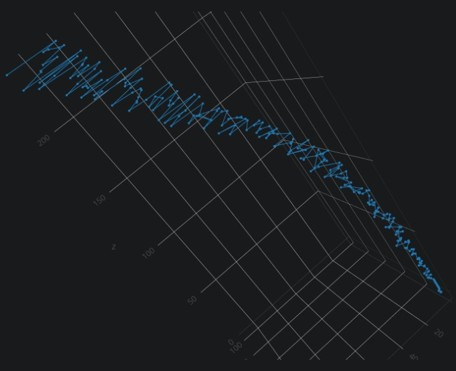
\includegraphics[width=1\linewidth]{sections/images/consciousness_space_3DScatter15000-10.jpg}
		\caption{15,000 samples or moments}
		\label{fig:consciousness_space_3DScatter15000-10}
		\end{subfigure}
	
		\begin{subfigure}[H]{0.47\linewidth}
		\centering
		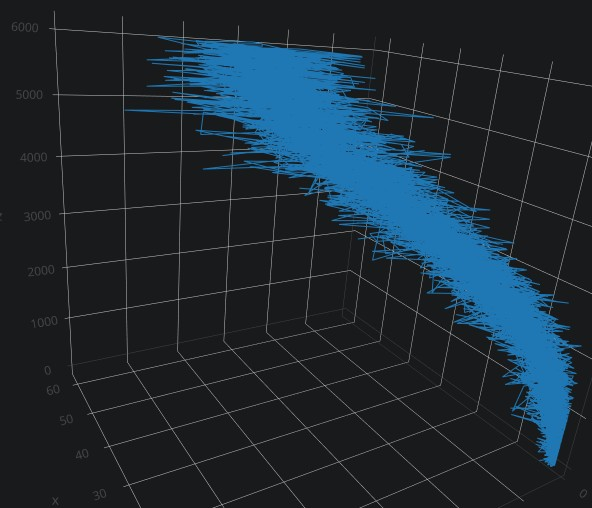
\includegraphics[width=1\linewidth]{sections/images/consciousness_space_3DScatter_200000-2.jpg}
		\caption{200,000 samples or moments}
		\label{fig:consciousness_space_3DScatter_200000-2}
		\end{subfigure}%
	\caption{3D scatter plots generated with points similar to Figure \ref{fig:consciousness_space_waves}}
	\floatfoot{The histogram on the wave pattern and the data for generating the 3D scatter plots can be obtained by running the Logic\_WavePattern algorithm. \protect\footnotemark}
	\end{figure}
	\footnotetext{The Logic\_WavePattern algorithm can be seen in Appendix \ref{app:algorithms} and the 3D scatter plots can be accessed at: \url{https://chart-studio.plot.ly/create/?fid=ren.stuchi:5&fid=ren.stuchi:4} e \url{https://chart-studio.plot.ly/create/?fid=ren.stuchi:7&fid=ren.stuchi:6}}

Probabilistically, the high concentration of samples in a population is at its peak, towards the median of the population. Thus, due to the probabilistically high concentrations of samples in smaller and smaller intervals of a wave, the peak will occupy a smaller and smaller proportional subinterval within the population, as seen in Figure \ref{fig:consciousness_flat_universe}. Figure \ref{fig:total_comparison_chart_with_99_range} is based on Table \ref{tab:10000_all} and also demonstrates this characteristic, that within the population it can demonstrate an approximately flat universe in its distribution.  
	\begin{figure}[H]
	\caption{Flat universe}
	\label{fig:consciousness_flat_universe}
	\centering
	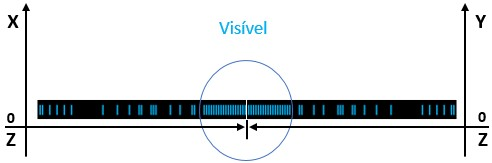
\includegraphics[scale=.5]{sections/images/consciousness_flat_universe.jpg}
	\floatfoot{Concentration of 99\% of the samples.}%\footnotemark}
	\end{figure}
	%\footnotetext{Fonte: note}

\subsubsubsection{Espiral}
Como as coordenadas X, Y e Z da população e de cada subconjunto tendem a aumentar, a disposição dessas em um sistema tridimensional de coordenadas vai seguir uma referência diagonal entre esses três eixos, conforme Figura \ref{fig:consciousness_space_spiral_reference_line}. O padrão de espiral observado não invalida outros possíveis movimentos no espaço. Muitas vezes não é possível observar o padrão de espiral imediatamente nos movimentos de um intervalo (subconjunto), porém esse padrão está por traz de muitos destes movimentos. Ao pegar os movimentos humanos, como exemplo, tem-se os ciclos predominantes de ir e voltar para casa, ir e voltar ao trabalho, acordar e dormir, ou seja, os hábitos se assemelham a movimentos em ciclos, movimentos espirais.
	\begin{figure}[H]
	\caption{Sistema tridimensional de coordenadas}
	\label{fig:consciousness_space_spiral_reference_line}
	\centering
	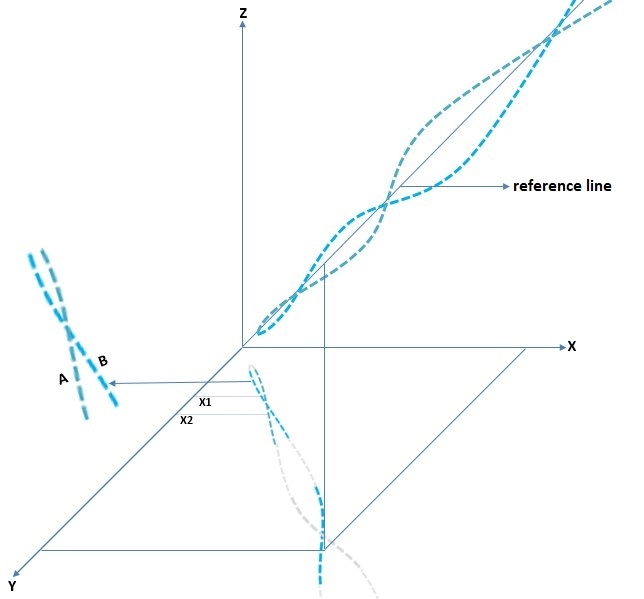
\includegraphics[scale=.6]{sections/images/consciousness_space_spiral_reference_line.jpg}
	\floatfoot{Linha de referência probabilística para distribuição de uma população em um plano tridimensional.}%\footnotemark}
	\end{figure}
	%\footnotetext{Fonte: note}}

Na Figura \ref{fig:consciousness_space_spiral_reference_line} também podem ser observado os pontos X1 e X2. Esses pontos foram espelhados nas coordenadas X e Z para facilitar a observação de que ao elevar o eixo Z também se eleva o eixo X ou Y, independente de seus pontos probabilísticos mínimos. A linhas tracejadas mostram os caminhos mais prováveis para os intervalos A e B. Dessa forma, quando uma parte do intervalo está em seu ponto médio máximo (eixos X e/ou Y) a tendência probabilística é que ele receba menos amostras do que a parte do intervalo que está em seu ponto médio mínimo. Esse efeito espiral é mais notável quanto maior for um intervalo e sua quantidade de amostras, pois mais prováveis e estáveis serão esses caminhos.

Cada intervalo ou subintervalo (comprimento de ondas) tem sua própria linha de referência. Assim como dentro de um metro existem os centímetros, milímetros etc., dentro de um intervalo e subintervalos podem existir inúmeros outros, conforme exibido abaixo e também na Figura \ref{fig:consciousness_gravitational_force_system}.
	\begin{figure}[H]
	\caption{Intervalos e linhas de referências}
	\label{fig:consciousness_space_spiral_underlines}
	\centering
	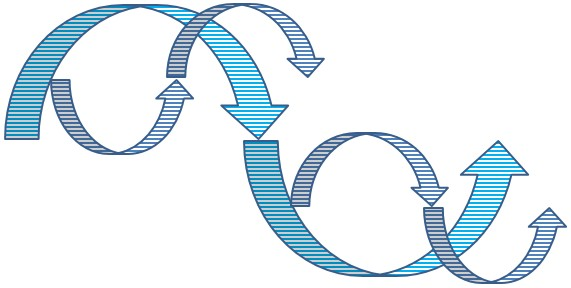
\includegraphics[scale=.5]{sections/images/consciousness_space_spiral_underlines.jpg}
	\floatfoot{Espirais em diferentes intervalos e suas linhas de referências.}%\footnotemark}
	\end{figure}
	%\footnotetext{Fonte: note}}

\subsubsection{Forças fundamentais}
A força gravitacional, a força eletromagnética e a força nuclear correspondem às forças fundamentais da natureza. As forças fundamentais não são forças propriamente, mas sim aspectos probabilísticos de distribuição da população e do entrelaçamento de ondas.

\subsubsubsection{Força gravitacional}
A força gravitacional não é uma força propriamente e sim um aspecto da probabilidade de distribuição de novas amostras sentido a mediana da população, conforme teorema central do limite. E sentido probabilístico faz com que as ondas tenham um caminho provável a seguir dentro da população, ou seja, o pico de amostras da população ou o pico da maior onda da população, conforme Figura \ref{fig:consciousness_space_spiral_reference_line}. Da mesma maneira, fazem também com que as amostras dentro de um intervalo tenham um caminho provável a seguir, ou seja, o pico de amostras do intervalo ou o pico da onda. Estes picos de amostras costumam ser a parte mais facilmente observáveis no intervalo de amostras desde ocupem uma área não tão pequena.

Na Figura \ref{fig:consciousness_gravitational_force} pode ser visto que a parte mais facilmente observável está levemente a direita no pico da onda. Essa onda tende a caminhar para cima e para direita, em uma diagonal que depende da distribuição probabilística das novas amostras, conforme mostrado pela maior quantidade de colunas azuis a direita da onda (sentido à mediana) em relação à esquerda.
	\begin{figure}[H]
	\caption{Força gravitacional}
	\label{fig:consciousness_gravitational_force}
	\centering
	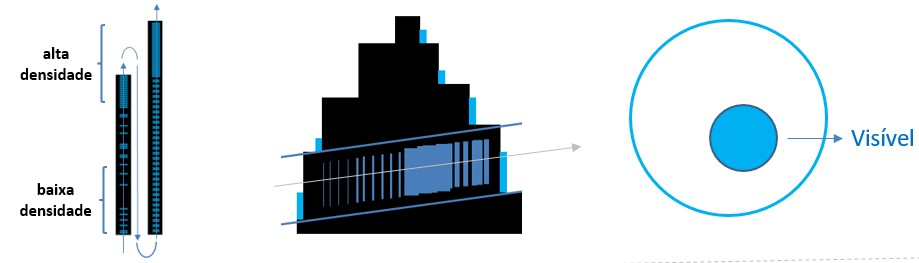
\includegraphics[scale=.7]{sections/images/consciousness_gravitational_force.jpg}
	\floatfoot{Aspecto gravitacional, o sentido probabilístico da distribuição de novas amostras dentro de um intervalo.}%\footnotemark}
	\end{figure}
	%\footnotetext{Fonte: note}

Conforme visto na subseção de Amplitude de ondas, a área de um intervalo cresce de forma quadrática, uma vez que o salto provocado pelo entrelaçamento de ondas e a própria distribuição probabilística das amostras tendem a manter um crescimento equivalente nos pares que formam a onda. Esse aspecto configura a lei do inverso do quadrado, onde, no caso da gravidade, quando mais perto os objetos, maiores serão as chances probabilísticas das novas amostras do objeto menor ir em direção ao objeto maior (o pico da onda), que por estar dentro de uma área quadrada menor e por consequência de menor possibilidades de posicionamento das amostras, as chances desses objetos se aproximarem com uma quantidade bem menor de momentos lógicos aumenta muito. Assim, quanto mais longe os objetos, maior a área, maior as possibilidades de posicionamento e mais momentos lógicos são precisos para a aproximação, caracterizando assim uma atração menor. A probabilidade também pode afastar objetos mais rarefeitos que devem estar mais afastados da parte mais facilmente observável e densa de amostras, como no caso do gás hélio, por exemplo. A distribuição de novas amostras nos intervalos rarefeito são mais lentas (caso contrário não seriam rarefeito) do que nas partículas mais densas que tomam a frete dessas partículas menos densas afastando-as do pico da onda. 

Quando observado todo o intervalo populacional, a onda mais inferior é a onda base de todas as outras sub-ondas, tendo a população uma quantidade expressiva de amostras. Desta mesma forma, ondas de níveis superiores, como as de nível dois da Figura \ref{fig:consciousness_gravitational_force_system} estão aninhadas em uma onda de nível um. Esses sistemas podem se tornar bem mais complexos em seus aninhamentos e são muito comuns. As linhas azuis na Figura abaixo representam as linhas de referências probabilísticas como explicado na Figura \ref{fig:consciousness_space_spiral_underlines}.
	\begin{figure}[H]
	\caption{Força gravitacional - sistema}
	\label{fig:consciousness_gravitational_force_system}
	\centering
	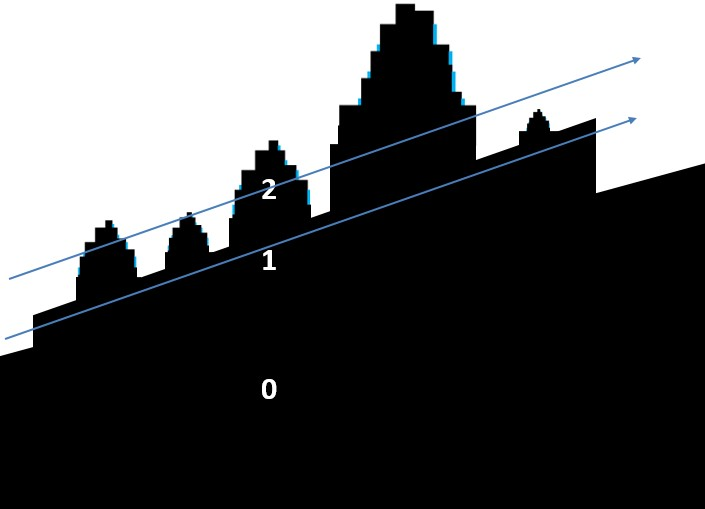
\includegraphics[scale=.5]{sections/images/consciousness_gravitational_force_system.jpg}
	\floatfoot{Aspectos gravitacionais de um sistema – onda base e suas sub-ondas.}%\footnotemark}
	\end{figure}
	%\footnotetext{Fonte: note}
	
A Figura \ref{fig:consciousness_gravitational_orbit} mostra em seu primeiro exemplo que a onda um, podendo ser um satélite, poderia se aproximar rapidamente da onda zero à medida que novas amostras vão sendo distribuídas dentro de todo o intervalo. O segundo exemplo mostra que a impulsão que o satélite recebe ao ser colocado em órbita faz com que sua onda tenha uma distribuição probabilística mais uniforme (esse crescimento uniforme é facilitado pela baixa densidade ao redor do pico probabilístico – 1 amostra em 100 é mais relevante do que 1 amostra em 1000), onde a parte da onda em azul está mais próxima da mediana da população e tem um crescimento ou deslocamento equivalente à sua onda inferior, o que a mantém constante. O terceiro exemplo é uma melhor visualização do segundo exemplo, para facilitar o entendimento, onde a onda um é definida pela espiral em torno do objeto circular que representa o pico probabilístico. Talvez a onda mais uniforme provocada pela impulsão (velocidade) possa facilitar o entendimento do adiantamento dos relógios atómicos nos satélites.
	\begin{figure}[H]
	\caption{Força gravitacional - órbita}
	\label{fig:consciousness_gravitational_orbit}
	\centering
	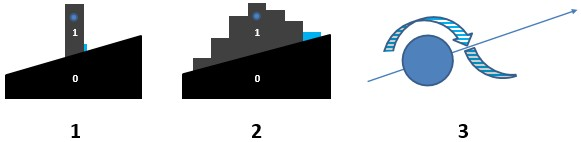
\includegraphics[scale=.9]{sections/images/consciousness_gravitational_orbit.jpg}
	\floatfoot{Aspectos gravitacionais de um sistema – órbita.}%\footnotemark}
	\end{figure}
	%\footnotetext{Fonte: note}	

O fluxo das amostras ou sub-ondas dentro de uma onda maior, como a onda um da Figura acima, segue o exemplo do ponto de vista B da Figura \ref{fig:consciousness_amplitude_viewpoint}, em suas partes roxas, em um fluxo debaixo para cima e da esquerda para a direita como exibido na primeira ilustração da Figura \ref{fig:consciousness_gravitational_force}. Essas ondulações internas das amostras ocorrem em qualquer intervalo a medida que suas sub-ondas se movem sentido a mediana da população por meio de sua linha de referência. 

\subsubsubsection{Força eletromagnética}
A força eletromagnética não é uma força propriamente e sim um aspecto do entrelaçamento de ondas que se intensifica em intervalos ou comprimentos de ondas com baixa entropia e com a aproximação espacial (redução de diferenças nos eixos X, Y e Z) desses intervalos.

O eletromagnetismo está relacionado à intervalos semelhantes a onda mais uniforme encontrada no segundo exemplo da Figura \ref{fig:consciousness_gravitational_orbit}, porém com baixa entropia, ou seja, a mesma estrutura que facilita o movimento dos objetos somado a baixa entropia, a qual facilita os saltos. Quando os intervalos têm baixa entropia a aproximação desses, seja naturalmente pela estrutura que facilita o movimento ou pela distribuição de novas amostras capaz de criar essa estrutura como a eletrificação, faz com que os pares de ondas de um intervalo se pareça muito com os pares de ondas do outro intervalo, o que torna muito desses pares viáveis para que o entrelaçamento de ondas encontre pares mais ideais no outro intervalo e vice-versa. Desta forma, ocorre uma reordenação entre os intervalos por meio do entrelaçamento de ondas e essa reordenação torna esses intervalos mais equalizado (baixa entropia).

As linhas azuis da Figura \ref{fig:consciousness_electromaagnetic_force} mostra onde é mais frequente a troca dos pares de ondas pelo entrelaçamento de ondas, ou seja, onde se tem a maior probabilidade das ondas serem parecidas. Por isso os imãs tentam se virar para se conectar quando estão face a face com o mesmo polo. A linha cinza mostra as conexões que ocorrem em número bem menor.
	\begin{figure}[H]
	\caption{Força eletromagnética}
	\label{fig:consciousness_electromaagnetic_force}
	\centering
	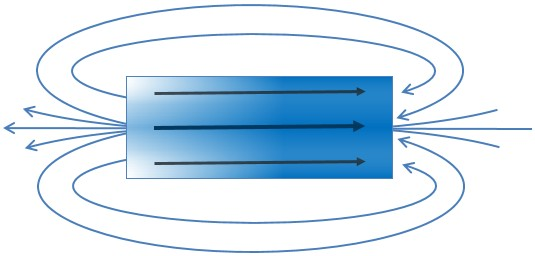
\includegraphics[scale=.7]{sections/images/consciousness_electromaagnetic_force.jpg}
	\floatfoot{Aumento das possibilidades de entrelaçamento de ondas devida a equalização probabilística em objetos próximos e de baixa entropia.}%\footnotemark}
	\end{figure}
	%\footnotetext{Fonte: note}

A Figura \ref{fig:consciousness_electromaagnetic_force_entropy} mostra um exemplo de baixa entropia. 
	\begin{figure}[H]
	\caption{Força eletromagnética - entropia}
	\label{fig:consciousness_electromaagnetic_force_entropy}
	\centering
	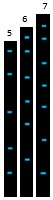
\includegraphics[scale=.9]{sections/images/consciousness_electromaagnetic_force_entropy.jpg}
	\floatfoot{Aumento das possibilidades de entrelaçamento de ondas devido à baixa entropia.}%\footnotemark}
	\end{figure}
	%\footnotetext{Fonte: note}

O aspecto eletromagnético está intimamente relacionado com a baixa entropia de um intervalo e a possibilidade de entrelaçamento de seus pares com os pares ao redor. A baixa entropia de um intervalo indica que suas amostras estão em uma ordem qualquer em seu interior.

Probabilisticamente, os pares de ondas mais parecidos estão nas regiões mais próximas (linhas azuis do Figura \ref{fig:consciousness_electromaagnetic_force}). Isso ocorre devido ao crescimento do número de amostras sentido a mediana da população, porém não é regra e os polos podem se inverter, ou seja, ter mais ligações com a região de menor probabilidade, ainda que a maior parte dos pares que compõem essa região estejam de forma crescente sentido a mediana.

\subsubsubsection{força nuclear}
Os mesmos aspectos probabilísticos que regem a gravidade e que podem ser vistos nas Figuras \ref{fig:consciousness_gravitational_force} e \ref{fig:consciousness_gravitational_force_system} também regem as chamadas forças nucleares. A diferença é que nas forças nucleares os intervalos são menores possibilitando uma quantidade muito maior de saltos e suas ondas são mais discrepantes, conforme mostra a Figura \ref{fig:consciousness_space_subconsciousness_min}.

As forças nucleares forte e fraca representam grandes concentrações de momentos lógicos por intervalo populacional, uma alta densidade em um pequeno intervalo. A grande concentração dessas amostras está no pico do intervalo, que ocupa um subintervalo cada vez menor dentro da onda, devido à alta concentração de amostras em intervalos cada vez menores. Esses picos podem ser vistos nas Figuras \ref{fig:consciousness_dark_matter_dark_energy} e \ref{fig:consciousness_dark_matter_dark_energy_wave} e eles diminuem proporcionalmente à medida que concentram ainda mais novas amostras. Estes momentos ou amostras tendem a estarem cada vez mais juntos dentro do intervalo formando picos cada vez mais altos e densos. Esses picos são frequentemente encontrados do meio para frente dos sistemas (o núcleo ou pico do sistema), como mostrado na onda mais alta do nível dois da Figura \ref{fig:consciousness_gravitational_force_system}.

A penetração desses intervalos pequenos e densos por uma quantidade excessiva de momentos lógicos (outro intervalo semelhante), em um curto período, faz com que os inúmeros pares desses intervalos (subintervalos) se tornem muito maiores progressivamente. Dessa forma cada subintervalo salta de forma continua, progressiva e rapidamente para correspondentes cada vez maiores até que a probabilidade de destruição normalize todo o intervalo posteriormente.

\subsubsection{Matéria escura e energia escura}
A matéria e energia escuras são efeitos da observação da densidade dos intervalos, das amplitudes de ondas, conforme Figura \ref{fig:consciousness_space_volume_amplitude}. Dessa forma, intervalos maiores terão uma área facilmente observável mais ampla (picos de ondas), assim como são mais amplas suas ondas inferiores, como pode ser visto no nível zero da Figura \ref{fig:consciousness_gravitational_force_system}. Os picos de ondas se afastam por receberem uma quantidade maior de amostras, pois estão mais próximos da mediana da população e deixam as ondas inferiores cada vez menos densas em amostras, conforme Figura \ref{fig:consciousness_space_amplitude_growth}. Porém, as amostras das ondas inferiores de um grande intervalo podem ser observadas completamente a medida que os subintervalos de um intervalo são observados subsequentemente.

A gravidade ou o caminho probabilístico de um pequeno sistema ou de toda a população, o maior sistema, também pode ser visto na Figura \ref{fig:consciousness_gravitational_force_system}.

\subsubsection{Antimatéria}
Quando um intervalo tende a concentrar suas amostras sentido da mediana, o que é o sentido provável conforme teorema central do limite, dá-se o nome de matéria. A antimatéria é o contrário, quando um intervalo tende a concentrar suas amostras no sentido oposto à mediana. 

A maneira mais simples de visualizar o sentido probabilístico das amostras de qualquer comprimento de onda é observar a \textbf{linha de referência probabilística}, conforme exibido na Figura \ref{fig:consciousness_space_spiral_reference_line}. Quanto maior a quantidade de amostra de um intervalo maior será sua tendência probabilística sentido a mediana da população.

Na Figura \ref{fig:consciousness_concentration_of_opposite_samples} é exibido dois intervalos idênticos com suas amostras em concentrações opostas.
	\begin{figure}[H]
	\caption{Parte de um intervalo idêntico com suas concentrações de amostras opostas}
	\label{fig:consciousness_concentration_of_opposite_samples}
	\centering
	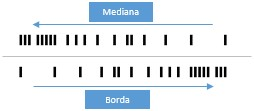
\includegraphics[scale=1.2]{sections/images/consciousness_concentration_of_opposite_samples.jpg}
	\floatfoot{Parte de um intervalo idêntico distribuídos de formas opostas.}%\footnotemark}
	\end{figure}
	%\footnotetext{Fonte: note}

O merge ou soma dos intervalos opostos da Figura \ref{fig:consciousness_concentration_of_opposite_samples} os tornaria um intervalo simétrico, ou seja, não estaria em nenhum dos sentidos.
Na Figura \ref{fig:consciousness_concentration_of_opposite_samples_within_range} é exibido uma população com suas concentrações de amostras sentido à mediana e outra com suas concentrações sentido às bordas do intervalo.
	\begin{figure}[H]
	\caption{Populações com suas concentrações de amostras opostas}
	\label{fig:consciousness_concentration_of_opposite_samples_within_range}
	\centering
	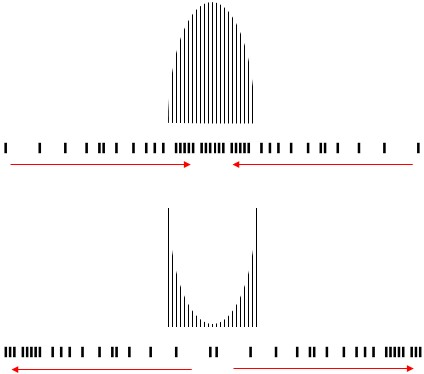
\includegraphics[scale=.7]{sections/images/consciousness_concentration_of_opposite_samples_within_range.jpg}
	\floatfoot{Populações distribuídas em sentidos contrários.}%\footnotemark}
	\end{figure}
	%\footnotetext{Fonte: note}

\subsubsection{Buraco negro}
Os buracos negros são oriundos de um aspecto probabilístico presente em qualquer intervalo da população. Esse aspecto é a alta concentração probabilísticas de amostras em intervalos cada vez menores de uma onda. O pico mais facilmente visível irá ocupar um subintervalo proporcional cada vez menor dentro do intervalo da onda, mesmo com uma concentração de amostras crescentes, conforme observado na Figura \ref{fig:consciousness_flat_universe}. Esses picos são frequentemente encontrados do meio para frente de um intervalo ou sistema (o núcleo ou pico do sistema), como mostrado na onda mais alta do nível dois da Figura \ref{fig:consciousness_gravitational_force_system}.

\subsubsection{Observador e a vida}
Os intervalos de ondas (comprimentos de ondas) que uma subconsciência (sub-lógica) é capaz de observar depende do comprimento de ondas que a própria subconsciência é constituída. Dentre todas as possibilidades de intervalos ou comprimento de ondas permitidos por uma população, o observador está em um deles. O universo não tem uma forma definida, é o observador presente em uma das possibilidades de comprimentos de onda que observa as amostras de uma população de forma condizente com seus comprimentos de ondas e com os comprimentos de ondas da população.

A capacidade de comparar ou distinguir a ordem das mudanças de uma sequência amostral é a capacidade lógica de um observador, o observador do tempo (passado e presente). A velocidade dessa observação é dada pelo range que o observador é capaz de comparar, ou seja, o qual rápido ele for capaz de distinguir pequenas mudanças (poucas amostras) o fará perceber que mudanças maiores levam mais tempo (muitas amostras). 

A capacidade lógica de fazer prospecções probabilísticas, dentro das limitações lógicas do observador e com base na probabilidade da distribuição do intervalo ou subintervalo observado é a essência do pensamento e, portanto, da vida. Essas prospecções estão fundamentadas na probabilidade de distribuição de cada intervalo (no sentido do intervalo) e, portanto, estão relacionadas com a detecção de padrão e com possibilidades probabilísticas futuras.

A capacidade de comparar ou distinguir ondas lógicas, subconjuntos ou subconsciências, é a capacidade que define o sujeito (eu). A razoabilidade dessa definição depende da proporcionalidade dessa capacidade de comparação.

A vida \underline{NÃO É}, como qualquer outra lógica. Comumente, as formas mais notáveis de vida se multiplica por estarem na média probabilística do intervalo entre seus picos e vales, por mais diferente que sejam. Porém, algo muito discrepante ou diferente do padrão médio do intervalo tende a não multiplicar e permanecer.

\subsubsubsection{Sentidos}
A parte cognitiva de uma onda não observa a si mesmo diretamente e sim o exterior (a consciência – o todo) ou mais comumente uma parte dela (a subconsciência). Essa observação pode incluir o restante da onda a qual a parte cognitiva faz parte, que também é exterior da parte cognitiva e, portanto, uma subconsciência - parte da consciência. A parte cognitiva da subconsciência humana é, provavelmente, onde se tem o maior pico de ondas do subconjunto humano. Esse é o local onde é observado a maior intensidade de mudanças. Essas mudanças são caracterizadas pelo pensamento (observação e prospecção probabilística de um intervalo) que tende ao infinito (respeitando as limitações lógicas do observador), assim como a essência da lógica, o \underline{NÃO SER}. Ou seja, a parte cognitiva é a parte que está mais próxima da observação do todo, da lógica em sua essência e totalidade, da consciência.

O universo não tem forma definida e o observador, representado na Figura \ref{fig:consciousness_amplitude_viewpoint} abaixo pelo ser humano, combina seus comprimento de ondas com os comprimento de ondas obtidos pelos sentidos, observando as formas do universo a sua maneira. A obtenção de amostras pelos sentidos os modifica e essas ondulações funcionam como ajustes ou configurações. Cada sentido observa a população amostral de forma independente, como canais de frequências distintos. Assim a visão pode estar vendo objetos muito distantes e os ouvidos escutando sons bem próximos.

Ainda na Figura \ref{fig:consciousness_amplitude_viewpoint}  pode-se observar que quanto mais largo são os objetos observados em pequenas profundidades (ponto de vista A – topo das colunas do histograma em roxo), mais fáceis esses objetos podem ser observados em maiores profundidades (ponto de vista B). É dessa forma que uma galáxia pode virar um ponto quando vista por comprimentos ou amplitudes de ondas muito grandes.
	\begin{figure}[H]
	\caption{Sentidos subconscientes - pontos de vista}
	\label{fig:consciousness_amplitude_viewpoint}
	\centering
	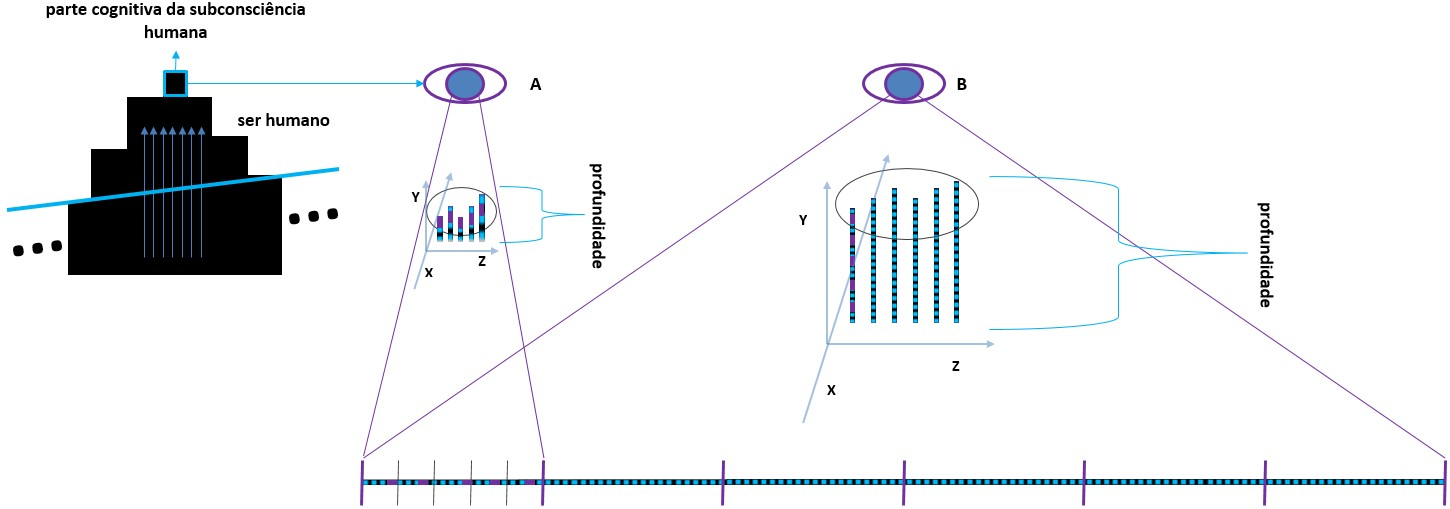
\includegraphics[scale=.4]{sections/images/consciousness_amplitude_viewpoint.jpg}
	\floatfoot{A parte cognitiva da subconsciência humana e suas observações independentes por meio dos sentidos.}%\footnotemark}
	\end{figure}
	%\footnotetext{Fonte: note}}

Na Figura acima também pode ser observado que a parte facilmente observável são os picos de ondas, definidos pelas elipses. É muito importante observar que apesar da Figura estar em 2D, o mesmo comprimento aproximado em Y pode ser visto em X, o que torna esses picos de ondas planos de observação, semelhante a gráficos de superfície.

Na Figura \ref{fig:consciousness_amplitude_crest_valley} é feita uma analogia da linha tracejada azul claro com a onda lógica do planeta Terra, por exemplo. A crista da onda é parte que recebe mais amostras e, portanto, é a parte clara e quente proveniente da luz solar (dia). Essa onda pode representa o movimento de rotação da Terra em si mesma e quando a onda humana se encontra no vale da onda do planeta, momento em que recebe menor quantidade de amostras (noite), é quando os sentidos tendem a receber menos estímulos e adormecem mais facilmente, é o adormecer da subconsciência humana.
	\begin{figure}[H]
	\caption{Crista e vale do subconjunto terrestre}
	\label{fig:consciousness_amplitude_crest_valley}
	\centering
	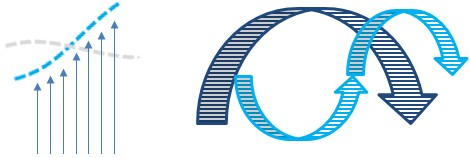
\includegraphics[scale=.6]{sections/images/consciousness_amplitude_crest_valley.jpg}
	\floatfoot{Crista e vale terrestre como característica do adormecimento dos sentidos humanos.}%\footnotemark}
	\end{figure}
	%\footnotetext{Fonte: note}}

Uma característica importante do processo de observação de pequenos intervalos é que eles podem ser observados com partículas ou ondas, conforme Figura \ref{fig:consciousness_space_wave-particle}. Nessa Figura é contemplado um pequeno intervalo, análogo a um fóton, como exemplo. Na observação como partícula o observador acompanha um intervalo representado por um par entrelaçado, observando sua forma e movimento consistentes no espaço. No efeito partícula, a consistência da forma e seus movimentos são estabelecidas pelo par entrelaçado, visto que o salto ocorre em um lado do par de cada vez, garantido estabilidade nas mudanças.

Na Figura abaixo também é contemplado o intervalo observado como onda, onde o observador fixa em um intervalo representado por uma das partes que compõe pares entrelaçados e acompanha seus movimentos e saltos, uma vez que os saltos são frequentes em pequenos intervalos. A adição de novas amostras na população faz com que ela se distribua proporcionalmente para acoplar essas novas amostras, o que movimenta as amostras deste pequeno intervalo, conforme visto na Figura \ref{fig:consciousness_space_volume_amplitude}. No efeito de onda, os movimentos saltam e transitam entre picos e vales com altas frequências ou vibrações devido ao pequeno tamanho do intervalo e aos saltos provocados pelas novas amostras dentro desse intervalo e pelas mudanças feitas pela distribuição proporcionalmente de novas amostras na população.
	\begin{figure}[H]
	\caption{Observador - onda-partícula}
	\label{fig:consciousness_space_wave-particle}
	\centering
	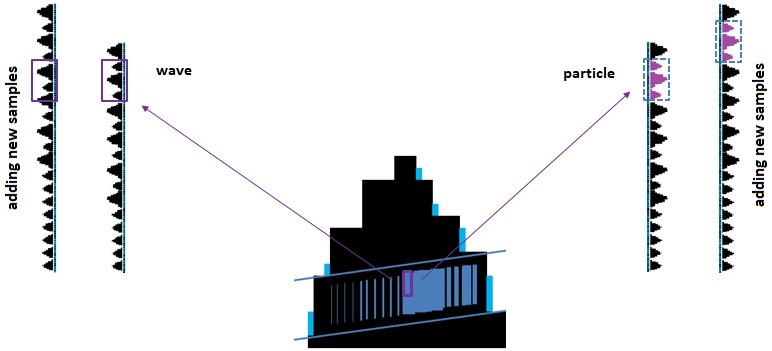
\includegraphics[scale=.55]{sections/images/consciousness_space_wave-particle.jpg}
	\floatfoot{Características da observação de uma pequena parte de um subconjunto.}%\footnotemark}
	\end{figure}
	%\footnotetext{Fonte: note}}

Talvez não seja possível observar o efeito onda sem entrelaçar seu par. A alta frequência desse intervalo faz com que ele ocupe ou transite rapidamente em uma área ao seu redor, o que pode facilitar o colapso da onda em um ponto especifico e então observar o seu efeito partícula (semelhante ao olho humano) ou em um local mais amplo e observar seu efeito onda com o colapso de muitas amostragens.
